\documentclass[a4,12pt,oneside]{book}
%\usepackage{times}
\usepackage{algorithmic} 
\usepackage[algoruled]{algorithm2e} 


\usepackage{setspace}
\usepackage{url}
\usepackage{geometry}
\usepackage{graphicx}
\usepackage{subfigure}
\usepackage{makeidx}
\usepackage{float}
\geometry{tmargin=1 in,  bmargin=1 in, lmargin=1.5 in,  rmargin= 1 in}
\setcounter{secnumdepth}{3}
\setcounter{tocdepth}{3}

\makeindex

\pagestyle{plain}
%\textwidth 6in
%\textheight 9in

\begin{titlepage}
 \title{\bfseries\huge TITLE}
  \author{A Dissertation Submitted in partial fulfillment of the degree of \\
    \\{\Large Master of Technology}\\in\\{\Large Computer Science}\\\\\\By\\\bf{STUDENT NAME}
  \vspace*{.2in}\\
    
\includegraphics[scale=0.5]{uoh.eps}\\ \\
	School of Computer and Information  Sciences\\
	University of Hyderabad, Gachibowli\\ 
	Hyderabad - 500046, India\\ \\
	Month, Year }
\end{titlepage}

\date{}

\renewenvironment{frontmatter}{\pagenumbering{roman}}{\newpage
  \pagenumbering{arabic}}
\renewcommand{\bibname}{Bibliography}
\newtheorem{algo}{Algorithm}[chapter]

\newenvironment{dedication}{
  \thispagestyle{empty}
  \clearpage\null\vfill
  \sl \hspace{1in}To,\\
  
  \hspace{1.5in}}{
  \vspace{3in}\vfill\null}


\def\prefacesection#1{%
  \chapter*{#1}
  \addcontentsline{toc}{chapter}{#1}
  \markboth{#1}{#1}}
\newenvironment{abstract}{\null\vfil\prefacesection{Abstract}}{\par\vfill\null}
\newenvironment{acknowledgments}{\null\vfil\prefacesection{Acknowledgments}}{\par\vfill\null}

\begin{document}
%\begin{large}
  \maketitle
 \onehalfspacing


\begin{frontmatter}
	{%certificate
	\thispagestyle{empty}
	\begin{center} 
		
\includegraphics[scale=0.5]{uoh.eps}
		\textbf{\Large CERTIFICATE}  
	\end{center}\vspace{.75in}

	{\sloppy This is to certify that the dissertation entitled ``\textbf{TITLE}'' 
    	submitted by \textbf{\mbox{STUDENT NAME}} bearing Reg. No. XXXXXXX, in partial fulfillment of the requirements for the award of Master of Technology in Computer Science, is a bona fide work carried out by him/her under my/our supervision and guidance.

	The dissertation has not been submitted previously in part or in full to this or any other University or Institution for the award of any degree or diploma. }\\ 

	\vspace{0.5in}
%	\parbox[t]{3in}
	{\flushright FACULTY NAME\\
	School of Computer and Information Sciences,\\
	University of Hyderabad\\}

	\vspace{1.0in}
%	\parbox[t]{3in}
	{\flushright Dean,\\
	School of Computer and Information Sciences,\\
	University of Hyderabad\\}
	}

\newpage
	{%declaration
	\thispagestyle{empty}
	\begin{center} 
		\textbf{\large DECLARATION}  
	\end{center}\vspace{.75in}

	{\sloppy I, \textbf{\mbox{NAME OF THE STUDENT}} hereby declare that this dissertation entitled ``\textbf{TITLE}'' submitted by me under the guidance and supervision of Professor/Dr. FACULTY NAME is a bona fide work. I also declare that it has not been submitted previously in part or in full to this or any other University or Institution for the award of any degree or diploma. }\\ \\ \\ \\ \\ \\

	{\flushleft Date:   } 
	{\flushright STUDENT NAME\\
	Reg. No.: XXXXXXXX\\
	\vspace{0.5in}
	Signature of the Student\\
	}
	}

    	\begin{dedication}
    	\thispagestyle{empty}
      		My Parents and Supervisor.
    	\end{dedication}
    
    	%\begin{acknowledgments}
      	%\paragraph\
I take this opportunity with immense pleasure to convey my gratitude to my supervisor, {\bf Ms. Anupama Potluri} who acted as a challenging captain coordinating all of our batch with great patience and invaluable suggestions. They really helped me to complete this task well before the stipulated time. She has always encouraged, supported, corrected and guided me during the project. This project happened to be one of my best journeys through core concepts of Computer Networks. The constant guidance of our supervisor helped me to develop both individually and professionally.\\

I can not get a better opportunity than this to thank profusely my senior {\bf Y. Jaya Lakshmi} with whose hard work my project literally became a cake walk. I would like to thank {\bf Tholoana Masupha} who is also part of this project. I am extreamly thankful to my lab mates {\bf B. Saritha, \bf B.Vishala and  \bf L. Ramprasad } for continuously inputting me with their valuable suggestions and being a source of encouragement at all possible times.  I would also like to thank the developers of {\bf ns2} for providing such a wonderful and robust software to work along with detailed documentation.\\

I am extremely grateful to our Head of Department, {\bf Prof. Arun Agarwal}, for providing excellent computing facilities and such a nice atmosphere for doing my project. I convey my heartfelt thanks to {\bf AI Lab staff} for their help in completing the project work successfully. \\

Last but not the least, I would like to express my heartful wishes to my beloved parents and my dear friends whose gracious solicitude helped me to complete this project successfully.  


\indent \indent \indent \indent \indent \indent \indent \indent \indent \indent \indent \indent \indent \indent \indent \indent \indent {\bf Sravanthi Bhavanam}
    	%\end{acknowledgments}
    
    	%\begin{abstract}
      	%\paragraph\
Mobile Adhoc Networks(MANETs) allow for infrastructure-less  mobile wireless networks to be established with minimal delay for deployment. The trend seen in applications of wireless services is that they make increasingly complex demands for Quality of Service(QoS). Thus, providing QoS in a MANET environment is becoming more important. However, QoS in MANETs is a challenging task, because of the inherent MANET limitations and properties. Some of the existing solutions are not scalable and have high signaling overhead. Some solutions are scalable but do not use the resources efficiently. Some solutions are simple but they do not even guarantee QoS and typically do not support multiple classes of service.
\paragraph\
Our proposed scheme is a cross-layer QoS-aware routing protocol that uses Diffserv model for data plane operations. It supports multiple classes of service and dynamically allocates resources for each QoS class. It reserves the resources for each flow and each flow is mapped to one of the QoS classes. The number of meters, policers and queues maintained per node are restricted to number of QoS levels only. So in this way it is scalable. As it reserves resources during route discovery process itself, it has less signaling overhead and has less latency to start data plane operations. To evaluate the performance of our scheme, we implemented it in the network simulator \textit{ns-2.29} by extending Dynamic Source Routing (DSR) protocol.
\paragraph\
Simulation results show that our scheme has achieved throughput close to ASAP while using fewer meters, policers and queues. Results also show that call acceptance ratio of our scheme is higher than ASAP. From the results we can also observe that our scheme gives QoS guarantee to the flows when congestion occurs whereas SWAN does not. Average end-to-end delay for our scheme is less than that of both ASAP and SWAN. Latency to start data plane operations is also acceptable in our scheme. Overall, we are performing better than ASAP and SWAN.
    	%\end{abstract}
    
    	\tableofcontents
    	\listoffigures
    	\listoftables
\end{frontmatter}
  
%\renewcommand{\baselinestretch}{1.7}
%\chapter{\label{chap:intro}Introduction}
%\paragraph\
 In computer networks the goal of QoS support is to achieve a more deterministic communication behavior, so that information carried by the network can be better preserved and network resources can be better utilized. QoS is an agreement or guarantee by the network to provide prespecified service attributes to the user in terms of delay, jitter(variance of delay), available bandwidth and probability of packet loss etc. QoS is essential to support real-time applications like VoIP, video conferencing, multimedia streaming etc. The Internet is, however, best-effort and does not provide any QoS. Many QoS models have emerged in recent times to support QoS in the Internet.

\section{QoS Models for Wired Networks}
\paragraph\
The two most popular QoS models for wired networks are
\begin{itemize}
\item Integrated services(Intserv).
\item Differentiated services(Diffserv).
\end{itemize}

\subsection{Integrated Services(Intserv)}
\paragraph\
The Integrated services model is the first standardized QoS model for the Internet. This model provides per flow QoS granularity. It reserves resources for each flow on the path by using Resource Reservation signaling protocol(RSVP) before commencing of the flow. The signaling messages carry QoS requirements of the flows. In this model per flow state information is maintained at the nodes and this information is refreshed periodically. At every node four basic components should be implemented. Those are signaling protocol, admission control, classifier and scheduler. It is well suited for meeting the dynamically changing needs of applications but it suffers from scalability problem.
 
\subsection{Differentiated Services(Diffserv)}
\paragraph\
 Diffserv is a fully distributed and stateless model. Instead of providing QoS at per flow granularity, Diffserv differentiates the traffic into a fixed number of classes. Diffserv aggregates a set of flows and applies a pre-defined behavior to that aggregate. So no state information for each flow is required to be maintained at any node. The network is divided into edge network and core network. The nodes at the edge of the network are responsible for classification of flows, policing them to ensure that the traffic complies with the agreement made by the service provider and marking the packets so that they can be differentiated in the core network. ToS field of the IP header is used for carrying marked codepoint. The nodes in the core network just check the codepoint of the packets and forward according to the per-hop behavior defined for that codepoint, making dataplane operations very efficient. 

\paragraph\
The raising popularity of multimedia applications among end users and the potential use of Mobile Adhoc Networks(MANETs) in civilian life have led to research interest in providing Quality of Service support in MANETs. We are also concentrated on this research area. In the following sections we discuss about MANETs and their features, what are the challenges for providing QoS in MANETs and the existing solutions and their drawbacks.

\section{Mobile Adhoc Networks(MANETs)}
\paragraph\
A Mobile Ad hoc Network (MANET) is a collection of wireless mobile nodes dynamically forming a temporary network without the use of any existing network infrastructure or centralized administration. It is a multihop wireless communication network in which each node can either act as a host or a router. MANETs represent future generation wireless networks, capable of being deployed quickly and economically at places lacking any infrastructure. These characteristics make MANETs more suitable for defense based applications, disaster relief operations and commertial applications.

\section{Challenges for Providing QoS in MANETs}
\paragraph\
Providing QoS in MANETs is challenging because of the following reasons:
\begin{itemize}
\item \textit{Dynamic network topology:} Nodes are mobile in the network. Link breaks occur due to mobility of nodes. The flows which are using these links are disturbed and latency is involved in finding a new route. It is also possible that a new route may not be found. Thus QoS can be violated for such flows.
\item \textit{Interference and Noise:} Because of the wireless medium there is more interference and noise. Due to this packet losses may be more. So we can not guarantee QoS.
\item \textit{Limited battery life:} Nodes are power constrained. So QoS solutions should not be too complex which consume more processing power of nodes.
\item  \textit{Bandwidth-constrained:} Bandwidth is very limited in wireless networks. The estimation of available bandwidth is very difficult because it not only depends on admitted flows in the channel, but also on the neighborhood nodes.
\end{itemize}

\section{QoS Models for MANETs}
\paragraph\
All the proposed models either use Intserv or Diffserv properties and these are mainly categorized as 
\begin{itemize}
\item Cross-layer solutions.
\item Independent solutions also known as frameworks.
\end{itemize}

\subsection{Cross-layer Solutions}
\paragraph\
QoS solutions can be provisioned at any layer in the protocol stack. Most existing schemes are at network layer. QoS-aware routing protocols will take QoS metrics as constraints to be satisfied, rather than trying to find the shortest path. Examples of these protocols are AQOR\cite{aqor}, ACOR\cite{acor}, QAODV\cite{qaodv} etc. A brief description of AQOR is presented in the next chapter.

\subsection{Independent Solutions}
\paragraph\
Instead of adding QoS to the routing or MAC layer, these schemes define separate QoS modules for signaling, admission control and scheduling etc. The main idea behind this is to separate functionality of each module so that these are independent to the routing or MAC protocols. Examples for these schemes are INSIGINA\cite{insignia}, ASAP\cite{asap} which are per flow QoS provisioning schemes and SWAN\cite{swan}, Diffserv framework\cite{diffframe} which are per class QoS provisioning schemes. We will discuss some of these frameworks in the next chapter.
 
\section{Motivation}
\paragraph\
From our literature survey, we find that the problems with existing QoS solutions for MANETs are
\begin{itemize}
\item Some are not scalable \cite{asap}, \cite{aqor}, \cite{insignia}.
\item A few have high signaling overhead \cite{asap}, \cite{ceqmm}.
\item There is no QoS guarantee\cite{swan}, \cite{asap}.
\item Many of the scalable schemes use static resource allocation which leads to waste of resources if there are no flows of tat QoS level\cite{diffframe}, \cite{ceqmm}, \cite{CLAD}.
\item Some of the schemes do not support multiple classes of services\cite{swan}, \cite{diffframe}.
\end{itemize}

\paragraph\
So, we proposed a cross-layer QoS aware routing protocol that supports multiple classes of service. It dynamically allocates resources for each QoS class. It reserves the resources for each flow and each flow is mapped to one of the QoS classes. The number of meters, policers and queues maintained per node are restricted to number of QoS levels only. So in this way it is scalable. As it reserves resources during route discovery process, it has less signaling overhead and the latency to start data plane operations is reduced. In addition, we use Diffserv principle of marking packets at the source(which is treated as an edge router) and simply enqueueing in the right queue at the intermediate routes speeding up processing in the data plane. To evaluate the performance of our scheme, we implemented the scheme in the network simulator \textit{ns-2.29} by extending Dynamic Source Routing (DSR) protocol which is an on-demand routing protocol for MANETs. We also ported the freely available implementations ASAP and SWAN to \textit{ns-2.29} for comparison of the performance of our scheme with them.
\paragraph\
Our simulation results show that the objectives with which we proposed our solution like scalability, high call acceptance ratio and QoS guarantee etc. are achieved.


\section{Organization of the Project Report}
\paragraph\
The rest of the project report is organized as follows: In Chapter 2, we present some of the  existing QoS solutions for MANETs with their advantages and disadvantages. In chapter 3, we present our proposal and implementation details of our proposal in network simulator \textit{ns-2.29}. Actually we have extended Dynamic Source Routing Protocol(DSR) to be QoS-aware. So in this chapter we present what are the extensions required and how we achieved them. Simulation results of our scheme, ASAP\cite{asap} and SWAN\cite{swan} are given in chapter 4. Simulation results show that our scheme performs better than ASAP and SWAN. Finally we conclude with chapter 5.
\chapter{\label{chap:survey}Related Work}
\paragraph\
  Flow monitoring protocols like NetFlow \cite{NetFlow} and sFlow \cite{sFlow} can provide   important information about traffic that 
  passes through a network. However, contemporary  networking with its 10Gbps and higher NICs is outpacing the ability to monitor them 
  efficiently. As data centers are getting virtualized with virtual software switches and scaling to thousands  of nodes, 
  it is an immediate requirement to have monitoring systems that can scale effectively. There are not many solutions proposed that 
  provide scalable flow monitoring in data center networks. In this chapter, we review some of the literature that deals with scalable 
  flow monitoring in data center networks.
  
  \section{Edge Monitoring and Collection for Cloud\\ (EMC2) \cite{emc2}} 
  \paragraph\
    Edge Monitoring and Collection for Cloud (EMC2) is a scalable network-wide monitoring service for data centers. 
    EMC2 stays inside the host computer  to monitor virtual switches. Monitoring at virtual switch is scalable due to 
    the distributed nature of the storage of the collected information.
    
  \subsection{Architecture}
    \begin{figure}[htb]
          \centering
          \includegraphics[scale=.35]{emc2.png}
          \caption{Architecture of EMC2 \cite{emc2}.} 
          \label{EMC2_arch}
    \end{figure}
    
    Figure \ref{EMC2_arch} shows the architecture of EMC2.

    \paragraph\
    EMC2 is a multi-threaded application that contains the following modules:
    \begin{enumerate}
     \item Flow-Table : Flow-Table is an in-memory 2-level hash table.
     \item NetFlowParser : It parses the NetFlow datagrams and updates the Flow-Table.
     %AP: ``It'' is a singular pronoun. Should be associated with a singular verb ``parses'' not the plural verb ``parse''. Similarly ``updates'' and not ``update''. They update, it updates, she updaes, he updates and so on. Please use the proper singular noun/pronoun and verb combinations.
     \item sFlowParser : It parses the sFlow datagrams and updates the Flow-Table.
     %AP: Missing articles: you need to say ``the sFlow'' and ``the Flow-Table'' since you are talking about a specific entity. If you are talking in general, then you need to use the article ``a'' or ``an'' depending on whether the word starts with a consonant or a vowel resp.
     \item NetFlowCollector : It accepts the NetFlow datagrams and creates the parser thread upon receiving NetFlow datagrams.
     \item sFlowCollector : It does the same task like the NetFlowCollector but for sFlow datagrams.
     \item FlowCollector : It invokes two thread -- NetFlowCollector and sFlowCollector -- for accepting flow datagrams.
  \end{enumerate}


    \subsubsection{Flow-Table}
      \paragraph\
	Flow-Table is a 2-level in-memory hash table. The primary key for the hash table is the Flow ID which is formed based on the 
	layer 3 source and destination addresses. Flow ID maps to another hash table where timestamp is the key and flow record is the value. Each flow record contains number of packets, number of bytes and optional path vector.
%AP: Overuse of hyphen (-). Please do not hyphenate everything.

    \subsubsection{NetFlowParser/sFlowParser}
      \paragraph\
	NetFlowCollector and sFlowCollector create these two parser threads upon receiving a NetFlow/sFlow datagram respectively. 
	These parser threads parse the datagram and update the Flow-Table. They also perform two important tasks:
	%AP: ``Parser threads'' is plural - hence use the plural verb ``perform'' not the singular ``performs''. Also, do not keep on saying ``Parser threads''. You can say ``They'' after the first one or two sentences. It is obvious that ``they'' refers to the preceding reference whatever that may be.

	\begin{enumerate}
	 \item Deduplication.
	 \item Data rate prediction in presence of sampling.
	\end{enumerate}
   %AP: Use enumerate wherever possible as it gives you numbering. Bullets are used in more special cases such as primarily in slides etc.
   
   \paragraph{Deduplication:}
       Deduplication prevents duplicate flow records from being added to the Flow-Table. 
       %AP: Please see how I have modified the above sentence from what you had written.
       It uses the following algorithm.
       
       
     \begin{algorithm}[H]
        \caption{Detect Duplicate Flow}
	\label{alg1}

	\begin{algorithmic}
	  \IF{$flow-ID$ not exist}

	      \STATE add flow to the flow table.
	      \RETURN 

	  \ELSE 

	      \IF {Same exporter}
		  \STATE update the flow table.
		  \RETURN 

	      \ELSE

	        \STATE report duplicate flow.
	        \STATE update path vector.
	        \RETURN 

	      \ENDIF

	  \ENDIF

	\end{algorithmic}

       \end{algorithm}

    \paragraph{Data Rate Prediction in Presence of Sampling:}
       Sampling rate is specified in flow datagrams. Parser thread predicts the data rate by multiplying  sampling rate with the length 
       of the packet.
   %AP: This is not clear to me still and as I said does not convey what you told me. I will defer modification of this until I have read the paper.
   
    \subsubsection{NetFlowCollector/sFlowCollector}
      NetFlowCollector/sFlowCollector are collector thread that wait %(AP: wait not waits)
      for new NetFlow or sFlow datagrams and spawn a new NetFlowParser/sFlowParser thread upon receiving a datagram.
      
    \subsection{Advantages and Limitations}
    The authors state the following advantages of EMC2:

    \begin{itemize}
     \item Scalable monitoring as EMC2 monitors host $vswitches$ in a distributed fashion by storing the information as flat files in
     those hosts itself instead of sending them to a centralized collector.
     %AP: I hope the above is correct in terms of the content of the paper.
    \end{itemize}
    
    However, flat files are not really built for scalability unlike many other distributed databases available today such as Cassandra, 
    Big Table etc.. Therefore, it is not clear how much of performance can be obtained by storing the information in flat files in the host 
    itself. Considering that most data centers work with SANs rather than local disks, this may not be as scalable as claimed.
    
    %AP: There is a real problem with your references. But, I will look at how you wrote your .bib file etc. on Monday.

   \section{Scalable Internet Traffic Measurement and Analysis with Hadoop \cite{Lee}}
   \paragraph\
   Hadoop \cite{hadoop} is a distributed computing platform that uses a distributed file system(HDFS) and MapReduce \cite{mapreduce} 
   programming model. A Hadoop cluster consists of 
   commodity hardware that can scale  to thousands of nodes to store huge amounts of data. It can perform massive data analytics operations on 
   the available data using MapReduce. Storing NetFlow data on Hadoop and analysis using MapReduce offers scalable traffic 
   measurement and analysis.
   %Nirmoy:add images to describe Hadoop cluster and MapReduce 
   %\subsection{Hadoop Architecture}
    \subsection{Architecture}
     Traffic measurement and analysis system with Hadoop consists of the following modules:
     \begin{enumerate}
      \item Traffic collector.
      \item IP packet and NetFlow reader in Hadoop.
      \item Analysis in MapReduce.
      \item Interactive query interface with Hive \cite{hive}.
     \end{enumerate}

     \subsubsection{Traffic collector}
     \paragraph\
     Traffic collection is done by a high-speed packet capture driver and load balancer. Load balancer forwards packets into
     multiple Hadoop data nodes evenly. Traffic collector also reads trace files stored on the disk and writes them into HDFS. 
     Trace files contains Netflow packets or IP packets in $libpcap$ format.
	
     \subsubsection{IP packet and NetFlow reader in Hadoop}
     \paragraph\
      Storing binary trace files into Hadoop specific sequence files needs more computation power as every packet has to be sequentially 
      read from the trace file and stored into HDFS. The authors have %AP: Authors is a plural, so the plural verb is ``have'' not ``has''.
      developed new Hadoop APIs to store trace files directly into HDFS. 
      As there is no distinct mark to find out the end of a packet record %AP: When you use the article ``a'' it means a single entity - you cannot say ``a packet records''.
      in $libpcap$ format, authors proposed a heuristic algorithm using timestamp-based bit pattern.

      \paragraph{Timestamp-based heuristic algorithm using MapReduce to identify packet records:}
	MapReduce job invokes multiple map tasks to process each	 HDFS block in parallel. 
	%AP: Do you mean that one block is processed in parallel or multiple blocks can be processed in parallel? If the latter, we have to change the above sentence? 
	Each of the map tasks follows these steps to identify the packet records in a HDFS block:
	\begin{enumerate}
	 \item Read two records using the $libpcap$ 16-byte header.
	 \item Check timestamp value, that should be within duration of captured time.
	 %AP: Cannot understand what you mean
	 \item Difference between wired packet length and captured length should be less than maximum packet length.
	 \item Check whether timestamp difference between the two packet records is within the defined
	 %AP: not ``within the define'' - you have to use past tense here.
	 threshold. 
	\end{enumerate}
	%AP: There is no way I can understand what the heuristic is and how it is helping from your description of the algorithm here. We will have to discuss this and I may have to re-write it to make a coherent algorithm.
	
	\subsubsection{Analysis in MapReduce}
	The authors have %AP: again, authors is plural and so you must use ``have'' - also, you must use the definite article ``the'' as the authors are defined - not just any authors in the world.
	implemented  analysis tools for processing IP packet as well as NetFlow packets using MapReduce algorithms. The tools implemented are:
	
	\begin{enumerate}
	 \item IP Layer analysis tools provide the following analysis jobs:
	      \begin{enumerate}
	       \item Host and port count statistics.
	       \item Periodic flow statistics.
	       \item Periodic sample traffic statistics.
	      \end{enumerate}
	 \item TCP layer analysis computes the following statistics:
	       \begin{enumerate}
	        \item RTT.
	        \item Retransmission.
	        \item Throughput.
	       \end{enumerate}
	\item NetFlow analysis provides 
	      \begin{enumerate}
	       \item Human readable flow statistics.
	       \item Aggregated flow statistics.
	       \item Top flows sorted by a key such as packet count or byte count. 
	      \end{enumerate}
	\end{enumerate}

      \subsubsection{Interactive query interface with Hive}
      Hive is a data warehousing system build on top of Hadoop that allows us to generate MapReduce jobs using SQL like query.
      IP analysis MapReduce jobs process NetFlow packets on HDFS and  store flow record and IP statistics into
      Hive tables. A user can then query the Hive tables using the interactive web-based user interface.
      
      \subsection{Advantages and Limitations}
      Advantages of Hadoop based traffic  measurement and analysis are 
	\begin{enumerate}
	  \item Scalable storage.
	  \item MapReduce operations on flow data.
	\end{enumerate}
      Disadvantages of Hadoop based traffic  measurement and analysis are
	\begin{enumerate}
	 \item Low response time- ``the fastest MapReduce job takes 15+ seconds" \cite{ha}.
	 \item Hadoop NameNode was a single point of failure which was solved in later version of 
	        Hadoop 2.0.0 with passive NameNodes.
	 \item Multiple NameNodes required to get high availability \cite{ha}.
	\end{enumerate}

	
      \section{\emph{nfdump} \cite{nfdump}}
      \paragraph\
      \emph{nfdump} provides a set of tools to capture and analyse NetFlow packets. The set of tools are :
      \begin{enumerate}
	\item \emph{nfcapd}
	\item \emph{nfdump}
	\item NfSen 
       \end{enumerate}

       \emph{nfcapd} reads data from the network and stores them into the disk. It also rotates %AP: rotates - remember the verb plural/singular rules - also, I am not anyway happy with the word rotate - dont you thnk CS has nice technical terms for such a behavior? Such as ''It treats the file as a circular queue to limit the size of the file``.
       the file to limit size of file.
      \emph{nfdump} allows $tcpdump$ style filter expression for processing NetFlow data stored by \emph{nfcapd} and displaying them on terminal or writing them into a file. NfSen gives a graphical overview of NetFlow data using RRDTool \cite{rrd};
        \begin{figure}[htb]
          \centering
          \includegraphics[scale=.35]{nfdump.png}
          \caption{Architecture of \emph{nfdump}.} 
	\end{figure}

	\subsection{Advantages and Limitations}
      \emph{nfdump} is suitable for small scale NetFlow analysis. In case of large scale NetFlow monitoring disk file based storage is not sufficient.
	
     \section{Packet Forwarding with \emph{netmap}\cite{spf}}
     \paragraph\
     This section describes about performance shortfalls of OpenVswitch \cite{ovs}, a study done by Luigi Rizzo and his team.
     \emph{netmap} \cite{netmap} is a framework to reduce the cost of moving traffic between the hardware and the host stack. As our network
     infrastructures moving from Fast Ethernet to Gigabit Ethernet and host stack APIs are not fast enough to handle such speed, 
     framework like \emph{netmap} is essential for such environment. %\emph{netmap} implements zero copy packet forwarding using shared memory
    % and data structures tune for fast packet receiving/forwarding.
    \paragraph\
    \emph{netmap} achieves efficient I/O by removing all unnecessary run time costs and system calls. \emph{netmap} exposes its API to userspace
    processes and provides a shadow copies of NIC rings.  Memory regions containing \emph{netmap} rings and packet buffers is shared with a
    process using $mmap$(). A user process can access NIC ring buffers directly, so transferring data can be done with zero copy operations.
    \emph{netmap} has a small \emph{libpcap} compatible API for migrating existing application.% to migrate to \emph{netmap}
     \paragraph\
     OpenVswitch is a multi-layer, OpenFlow \cite{openflow} compliant virtual switch designed to automate network through programmatic extensions. OpenVswitch is currently 
     heavily used for network virtualization. So performance analysis of OpenVswitch is critical as we are modifying it to support
     scalable flow monitoring.
     
     Authors have used \emph{netmap} for \emph{libpcap} alternative to improve the performance of OpenVswitch from 65 Kpps to 1.3 Mpps.
     After resolving few architectural limitations of OpenVswitch, authors have able to get three times performance improvement.
     Table \ref{openvswitch-perf} shows the performance of OpenVswitch under various environment.\\
     \begin{table}[th]   
      \centering
      \begin{tabular}{|l|r|}
        \hline
        {\bf Configuration} & {\bf Kpps}  \\ \hline      
         Linux userspace     & 50          \\ \hline 
         FreeBSD userspace   & 65          \\ \hline 
         Linux Kernel        & 300         \\ \hline 
         Optimize OpenVswitch + FreeBSD & 790  \\ \hline
         Optimize OpenVswitch + FreeBSD + \emph{netmap} & 3050  \\ \hline
      
         \end{tabular}
       \caption{OpenVswitch Performance with \emph{netmap}}
       \label{openvswitch-perf}
     \end{table}
     So from this table we can easily find impressive performance gain by OpenVswitch using \emph{netmap}.
     This paper \cite{spf} also gives us internal architecture of OpenVswitch that helped to modify OpenVswitch
     for our second approach to have scalable flow monitoring with $Vswitch$.
     
     
     %\section{Virtual I/O for Virtual Machines with \emph{virtio} \cite{virtio}}
     %\paragraph\
      
     
     
     
      \section{Summary}
      In this section I have discussed  available solutions for scalable flow monitoring. The issues with current solutions are 
      \begin{enumerate}
       \item Lack of scalable storage \cite{emc2} \cite{nfdump}.
       \item Lack of high availability data storage \cite{Lee}.
       \item Real-time flow analysis is difficult with current systems \cite{Lee}.  
      \end{enumerate}

      
      In the next chapter I describe the design and implementation of modified \emph{ntop}(a NetFlow collector) that 
      tries to solve a few of these issues.
      

%\chapter{\label{chap:our-idea} Proposal and Implementation}
%\paragraph\
In this chapter, I describe the proposed protocol \textit{QoS aware Routing using Diffserv principles\cite{thesis}} and I present the design of the protocol. I also specify my contribution to that protocol in the implementation part. To compare our scheme with respect to parameters like call acceptance ratio, latency to start dataplane operations, packet delivery ratio and throughput, I have ported ASAP\cite{asap} and SWAN\cite{swan}, which were already described in the previous chapter, to network simulator \textit{ns-2.29}.
%AP: Please put ns-2.29 in italics everywhere.

\section{QoS aware Routing using Diffserv Principles\cite{thesis}}
\paragraph\
This scheme is proposed by Jaya Laksmi et al.\cite{QoSdiff} to take advantage of both Intserv and Diffserv. It provides
\begin{enumerate}
\item Scalability in terms of meters and policers used.
\item Dynamic resource allocation per flow.
\item Per QoS-level policing and metering.
\item Multiple classes of service.
\item Soft state resource release.
\item Low signaling overhead.
\end{enumerate}

\paragraph\
In this scheme, the source acts as an edge router and others act as core routers. Service level agreements like Committed Information Rate(CIR), Peak Information Rate(PIR) are configured dynamically. An assumption in this scheme is that every node knows the existing QoS levels and their corresponding Diffserv Code Points(DSCP).

\subsection{Routing Algorithm}
\paragraph*{Route discovery}
To admit a real time flow, the source first checks its routing table. If it does not have any route for this flow, then it will do admission control. If admission control succeeds, the source broadcasts QRREQ packet. QRREQ carries minimum and maximum bandwidth requirements of the application. Intermediate nodes which receive this QRREQ will do admission control and if it succeeds they will rebroadcast the QRREQ packet; otherwise they simply discard the packet. If admission control succeeds at the destination, it will give a reply, QRREP, to the first received QRREQ in the reverse path, after populating its routing table and session table. Session table is a table that contains session ID of that flow, source ID , the minimum bandwidth reserved, length of the path and initial DSCP value. The amount of reserved bandwidth is deducted from available bandwidth and added to the corresponding QoS level. Every intermediate node on the path checks for admission control once again when forwarding the reply. If it succeeds, the node adds the minimum bandwidth to the bandwidth for that QoS level and deducts it from its available bandwidth. Otherwise, the node at which admission control fails will set the admission control (\textit{ac}) bit in the QRREP and just forwards it towards the source. The nodes downstream to that node will simply forward the reply to the source without processing it further. If the source gets QRREP with \textit{ac} bit set, then it will initiate the route discovery process again. Otherwise, it populates its routing table and session table and starts transmitting data.

\paragraph*{Resource maintenance}
Reserved resources are refreshed through data plane operations. If the flow is completed or a route break occurs and the flow no longer uses a node, the soft state timer on the reservation expires and the bandwidth of that flow is returned to available bandwidth.

\paragraph*{Route maintenance}
When a route break occurs while forwarding data, the node which precedes the broken link sends RERR message to the source after releasing resources of that flow and resources of all the other flows which are using that path. After receiving RERR, the source restarts the route discovery process.

\subsection{Data Plane Operation}
After finding the route, the source marks the data packets with the corresponding initial diffserv code point. After applying metering and policing these packets are again remarked with different drop precedences based on whether they are in- or out-of-profile. Now these are enqueued into the corresponding queues. The marking and conditioning is done only at the source node as it is the edge router. The intermediate nodes, which are like core routers, just check the DSCP value in the packets and enqueue into the corresponding queues. When congestion occurs, the packets will be dropped according to drop precedence. Weighted Round Robin(WRR) mechanism is used to schedule the packets.

The protocol is implemented in the network simulator \textit{ns-2.29} by extending the Dynamic Source Routing protocol\cite{dsr}.

\section{Design of the Protocol}
\paragraph\
The class diagram of the whole protocol is given in fig\ref{classdiagram}. All the classes are specific to \textit{ns-2.29} implementation of DSR\cite{dsr} as we are extending DSR protocol to implement our protocol. \textit{DSRAgent} is the main class which implements all functionalities like route discovery and route maintenance.
%We will explain about each of these classes in the remaining sections.
\begin{figure}[!h]
\centering
\includegraphics[scale=.77]{figures/classdiagram.eps}
\caption{Class diagram.}
\label{classdiagram}
\end{figure}

\paragraph\
Jayalakshmi had defined QRREQ and QRREP packets by extending normal RREQ and RREP packets of DSR\cite{dsr}. The extra fields in the QRREQ packet are minimum bandwidth, maximum bandwidth, bottleneck bandwidth and session ID. The QRREP packet contains bottleneck bandwidth, session ID and initial DSCP of the flow. She had implemented the generation and propagation of these QRREQs and QRREPs.

\paragraph\
Tholoana Masupha had defined the new interface queue \textit{dsrDiff} for our protocol. For this purpose she has defined a new class - \textit{dsrDiff}. This class is also useful to differentiate the edge router functionality from the core router functionality. She has defined four QoS levels of service based on the application bandwidth requirements.

\paragraph\
My contribution to the protocol is the implementation of:
\begin{enumerate}
\item Route request table modification.
\item Admission control functionality.
\item New route cache implementation.
\item Dynamic allocation of resources to each class. 
\item Soft state management of session records.
\item Data plane processing.
\end{enumerate}

The remaining sections of this chapter describe each of the above in detail. First, we describe the way DSR handles each of these. Then, we describe the modifications needed to support QoS extensions and how they have been designed and implemented.

\section{Request Table Modification}
\paragraph\
In DSR, if many flows start at the same time from the same source to the same destination, route discovery is initiated for that destination only once. The source checks to see if any request is outstanding for this destination in its request table. If so, it does not initiate route discovery. But in our protocol the source should initiate route discovery for all flows because we need to reserve the resources for every flow. So to achieve this, we have added session ID field to the request table. The source checks its routing table and compares the destination ID and session ID of the current flow with those which are destined to the same node. If no matching entry is found, then the source initiates route discovery for the new flow. If an exact match exists, then, the data packets can be forwarded using that route cache entry.

\section{Admission Control}
\paragraph\
DSR is a best-effort routing protocol. It does not require any available bandwidth information at that
%AP: you have used doesn't in many places. Please remember not to do so in formal documents.
 node. But our protocol is QoS-aware and it should guarantee the flows. It should not admit the flows for which nodes do not have sufficient bandwidth. So to do this admission control, every node should know the available banwidth at that node. We are maintaining the available bandwidth value in the MAC layer. As shown in the class diagram \ref{classdiagram} we have added available bandwidth field in the MAC class. This value is initialized to the link bandwidth. As bandwidth is reserved and released from flows, this value is changed.

\section{New Route Cache Implementation}
\paragraph\
In DSR, every node has its own route cache. The route cache can store the learned source routes. These routes can be used by intermediate nodes. Intermediate nodes can give reply by using these cached route entries. These route entries are refreshed through data plane operations. The node can also remove the routes when it learns about the broken link by getting RERR packet. If the route is not used by any flow, then, after timeout period these routes are deleted from the route cache.

\paragraph*{Implementation Details} 
In \textit{ns-2.29} implementation of DSR, three types of caches are defined. Those are \textit{SimpleCache}, \textit{LinkCache}, \textit{MobiCache}. By default \textit{DSRAgent} chooses \textit{MobiCache}. \textit{MobiCache} stores the whole source route in it. It defines two caches - primary cache and secondary cache. Primary cache is used by the source and the destination nodes. Intermediate nodes use secondary cache to store the routes. As shown in the class diagram \ref{classdiagram} \textit{MobiCache} is derived from \textit{RouteCache} which is an abstract class. Primary cache and secondary caches are objects of \textit{Cache} class. \textit{Cache} class is a set of objects of \textit{Path} class. The \textit{Path} class is an array of nodeIDs which represent the path for a destination that this node is aware of. Each \textit{Path} object in the \textit{Cache} object represents the route to all the various nodes that comprise this path.

\paragraph\
In our protocol we need to store the session information, in addition to the route, in the cache for a flow. Session information tells how much bandwidth to release from which QoS class for that flow. So, this session information should be maintained per flow. As explained before, the cache maintains total route to the destination in one path object. So, if there are multiple flows to the same destination for which the same route is found after QoS route discovery, we need to maintain the list of associated session records for the same path object. Also, if there are data flows to any of the other nodes on the route, these are also part of the same path object and hence session records for all these flows are also maintained as part of the same path object. The algorithm for adding route and session record is given in Algorithm 1.

\begin{algorithm} [!hbt]
\caption{\textit{\textbf{addRoute() function}}}
\begin{algorithmic}[1]
%\STATE	$addRoute(newpath, sessionrecord)$
\FOR	{each entry in the cache}
\STATE	compare the newpath with the cache entry.
\IF	{cache entry is NULL}
\STATE	add path to the cache.
\STATE	$AddSRecordatBegining(sessionrecord)$
\STATE	$return$
\ELSIF	{total newpath or some part of the new path matches the total or part of cachepath}
\IF	{$newpath.length() < cachepath.length())$}
\STATE	$position \leftarrow GetSRecordPosition(sessionrecord)$
\STATE	$AddSRecordatPosition(sessionrecord, position)$
\STATE	$return$
\ELSIF	{$newpath.length() > cachepath.length())$}
\STATE	append remaining path to the cachepath.
\STATE	$AddSRecordatEnd(sessionrecord)$
\STATE	$return$
\ELSE
\STATE	$AddSRecordatEnd(sessionrecord)$
\STATE	$return$
\ENDIF
\ENDIF
%\ENDIF
\ENDFOR
\end{algorithmic}
\end{algorithm}

\paragraph\
Whenever any intermediate node on the path moves away, the nodes beyond this node are no longer reachable. Hence in DSR implementation, when this happens, the path is truncated up to the node that has   moved away. In addition to this, in DiffQ-DSR, every node should delete the session records of these nodes and reclaim the bandwidth to the available bandwidth. To achieve this, in each session record, we maintain the length of the path to the destiantion of that session. If, after truncation, the length of the path is less than the length in a session record, the destination of that session is no longer reachable. So, we walk through the session list and delete all session records whose path length is greater than the current path length. The session list is maintained in a sorted order to accomplish this efficiently. The following figures show all this functionality clearly.
%AP: I am still not happy with the description above. Will discuss it with you tomorrow. But, try to rewrite again and show me the new version, if you can, tomorrow.

\begin{figure}
\centering
\includegraphics[scale=.45]{figures/s1.eps}
\caption{Flow f1 starts between s1 and 2 and corresponding cache entries.}
\label{s1}
\end{figure}

\begin{figure}[!h]
\centering
\includegraphics[scale=.45]{figures/s2.eps}
\caption{Flow f2 starts between s1 and D and corresponding cache entries.}
\label{s2}
\end{figure}

\begin{figure}[!h]
\centering
\includegraphics[scale=.45]{figures/s3.eps}
\caption{Flow f3 initiates between s1 and 3 and corresponding cache entries}
\label{s3}
\end{figure}

\begin{figure}[!h]
\centering
\includegraphics[scale=.45]{figures/s4.eps}
\caption{After processing of RERR cache entries.}
\label{s4}
\end{figure}

\paragraph\
In Figure \ref{s1}, consider that there is a flow f1 between s1 and 2. If s1 finds the path \textit{s1-1-2} for the flow f1, then it stores the path \textit{s1-1-2} and the associated session record s2 in its cache. Now after some time, a flow f2 starts between s1 and D and consider that s1 finds that the path \textit{s1-1-2-3-D} satisfies the QoS requirements for the flow f2. Then  while storing this path in its cache, s1 finds that it has already some part of the path in its cache and it just appends the remaining path \textit{3-D} to that path. S1 adds the session record \textit{sd} at the end of the session list as its length of the path value is greater than the previous session record s2's length of the path value. This is shown in Figure \ref{s2}. Now again consider that there is a flow f3 between s1 and 3 and the path satisfying the flow f3's QoS requirements is \textit{s1-1-2-3}. Whenever s1 tries to store this path, it finds that it has already that path in its cache. Then s1 inserts the session record s3 in between s2 and sd in the session list as s3's length field value is 4. This is shown in Figure \ref{s3}. Now if the node 3 moves away, the source gets the route error and it truncates the path from \textit{3-D}. Now the updated path length is 3. So s1 deletes all the session records whose length field is greater than this updated path length. This is shown in Figure \ref{s4}. So by getting RERR for the flow f2 only, s1 initiates the route discovery for f3 even before it gets RERR for this flow. By doing this we can reduce the packet loss.

\paragraph\
To implement the above functionality we defined two new classes: \textit{QPath} and \textit{SessionRecord}. \textit{QPath} class is derived from \textit{Path} class because we need all the functionality that \textit{Path} class provides. To associate the session list with the path, we have defined container relationship between the SessionRecordList class and QPath class. The class \textit{SessionRecord} contains the fields source Id, session ID, bottleneck bandwidth, DSCP and length of the path. All these classes and the relationships between them is shown %AP: there is no such word as showed - it is shown. Please change it.
 in Figure \ref{classdiagram} 

\paragraph\
To store the session records, we need to know the position where to insert because we are maintaining session records in the sorted order. The algorithm for this functionality is given in Algorithm 2.

%$GetSRecordPosition()$
\begin{algorithm} [!hbt]
\caption{\textit{\textbf{GetSRecordPosition() function}}}
\begin{algorithmic}[1]
\FOR	{each SRecord in SessionList}
\IF	{$SRecord.length <= sessionrecord.length$}
\STATE	$position \leftarrow position+1$
\ELSE
\STATE	return position
\ENDIF
\ENDFOR
\end{algorithmic}
\end{algorithm}

\section{Route Maintenance}
Whenever a route break occurs, the node which precedes the broken link will send RERR to the source. This RERR packet contains the IP addresses of the two nodes between which the link is broken. The processing of RERR is given in Algorithm 3. In this algorithm $DeleteSessionList(n+1)$ function deletes all the session records whose length fields are greater than $n+1$ value.  $n+1$ represents the updated path length.


%$processBrokenLink(RERRpacket)$
\begin{algorithm} [!hbt]
\caption{\textit{\textbf{processBrokenLink() function}}}
\begin{algorithmic}[1]
%\STATE $processBrokenLink(RERRpacket)$
\FOR	{each path in the cache}
\STATE	$n \leftarrow 0$
\WHILE	{$ n < path.length() $}
\IF	{path[n] = RERRpacket.fromnode and path[n+1] = RERRpacket.tonode}
\IF	{$n = 0$}
\STATE	delete the whole path
\ELSE
\STATE	truncate the path from n+1 node
\ENDIF
\STATE	$DeleteSessionList(n+1)$
\STATE	break
\ENDIF
\STATE	$n \leftarrow n +1$
\ENDWHILE
\ENDFOR
\end{algorithmic}
\end{algorithm}

\section{Session Record Maintenance}
\paragraph\
SessionRecordTimer class maintains the soft state of the session records. It checks the sessionrecord list periodically. If any session record timer expires that session record will be deleted and resources are released. This functionality is given in Algorithms 4 and 5.

%$SessionListCheck()$
\begin{algorithm} [!hbt]
\caption{\textit{\textbf{sessionListCheck() function}}}
\begin{algorithmic}[1]
\FOR	{each entry in the cache}
\STATE	$temp \leftarrow GetFirstSRecord()$
\WHILE	{$ temp \neq NULL$}
\IF	{$(currenttime - temp.SRTime) > SessionTimeout$}
\STATE	$temp1 \leftarrow GetNextSRecord()$
\STATE	$releaseResources(temp)$
\STATE	$DeleteSRecord(temp)$
\STATE	$temp \leftarrow temp1$
\ELSE
\STATE	$temp \leftarrow GetNextSRecord()$
\ENDIF
\ENDWHILE
\ENDFOR
\end{algorithmic}
\end{algorithm}

\begin{algorithm} [!hbt]
\caption{\textit{\textbf{releaseResources() function}}}
\begin{algorithmic}[1]
%\STATE	$releaseResources(sessionrecord)$
\STATE	$addtoAvailBW(sessionrecord.SRbbw)$
\STATE	$deductFromQoSlevel(sessionrecord.SRbbw)$
\STATE	$minbw \leftarrow getminBW(sessionrecord.SRdscp)$
\STATE	$maxbw \leftarrow getmaxBW(sessionrecord.SRdscp)$
\STATE	$deductFromCIR(minbw)$
\STATE	$deductFromPIR(maxbw)$
\STATE	return
\end{algorithmic}
\end{algorithm}

\paragraph\
These session records are refreshed through the dataplane operations. For this purpose we have added new DSR option to hold session ID in data plane packets. The algorithm for this is presented in Algorithm 6.

%$refreshSessionRecord()$
\begin{algorithm} [!hbt]
\caption{\textit{\textbf{refreshSessionRecord() function}}}
\begin{algorithmic}[1]
%\STATE $refreshSessionRecord(src, sid)$
\FOR	{each entry in the cache}
\STATE	$temp \leftarrow GetFirstSRecord()$
\WHILE	{$ temp \neq NULL$}
\IF	{$temp.SRsrc = src\ and\ temp.SRsid = sid$}
\STATE	$temp.SRTime = currenttime$
\STATE	$return$
\ELSE
\STATE	$temp \leftarrow GetNextSRecord()$
\ENDIF
\ENDWHILE
\ENDFOR
\end{algorithmic}
\end{algorithm}

\section{Dynamic Resource Allocation}
\paragraph\
In general Diffserv implementation, the metering values Committed Information Rate(CIR) and Peak Information Rate(PIR) for the QoS classes are fixed and these are assigned to each QoS class at the begining.  %AP: you dont say starting in such places - use the word beginning instead of starting.
But in our protocol, whenever a flow of that particular QoS class is admitted, then the CIR and PIR values are assigned to that class. These metering values are changed dynamically according to the flows admitted to that class. While processing QRREP every node adds the minimum bandwidth requirement of the flow to the CIR of the QoS class to which that flow belongs. In the same way maximum bandwidth requirement of the flow is added to the PIR.

\section{Data Plane Operation}
\paragraph\
In DSR, the data packet carries the whole source route from the source to the destination which is copied from the route cache. Intermediate nodes which get this data packet add the source route to their cache if they do not have it. Otherwise, they simply refresh the route. Instead of carrying the whole source route, the data packet carries flow ID in the new extension of DSR. DSR uses only one interface queue for all the flows to enqueue the packets before they are transmitted by the network interface.

\paragraph\
In our protocol, every data packet carries the whole source route and to refresh the session records we have added session ID option to the DSR header. At the source node each data packet is metered, marked and policed. Every intermediate node just checks the marked value and enqueues it to the corresponding queue. We have defined four QoS classes of service and three drop precedences for each QoS class. So we need to have four physical queues corresponding to the four QoS classes and each physical queue should have three virtual queues corresponding to the three drop precedences. We are using RED queue management.

\paragraph\
To implement the above functionality, we are using the classes \textit{DSRPolicy}, \textit{dsrredQueue}, \textit{dsrREDQueue}, \textit{QOSClass} and \textit{dsrDiff}. The relation between all these classes is shown in Figure \ref{classdiagram}. \textit{dsrDiff} class differentiates the edge router functionality and core router functionality. \textit{dsrREDQueue} class provides four physical queues and the class \textit{dsrredQueue} provides three virtual queues. \textit{DSRPolicy} class implements all the functionality of marking, metering and policing.

Algorithm 7 gives the data plane operation in our protocol  

\begin{algorithm} [!hbt]
\caption{\textit{\textbf{Data plane operation}}}
\begin{algorithmic}[1]
\STATE $packet \leftarrow recv(dataPacket)$
\IF     {$nodeID = packet.dest$}
\STATE	$refreshSessionRecord(packet.src, packet.sessionID)$
\STATE	$acceptPacket(packet)$
\ELSIF	{$nodeID = packet.src$}
\STATE	$path \leftarrow findroute(packet.dest, packet.src, packet.sessionID)$
\IF	{$path \neq NULL$}
\STATE	$packet.path \leftarrow path$
\STATE	$mark(packet)$
\STATE	$applyMetering(packet)$
\STATE	$applyPolicer(packet)$
\STATE	$enqueue(packet)$
\ELSE
\STATE	$getQRouteforPacket(packet)$
\ENDIF
\ELSE	\STATE \COMMENT {/* At intermediate nodes */}
\STATE	$refreshSessionRecord(packet.src, packet.sessionID)$
\STATE	$enqueue(packet)$
%\ENDIF
\ENDIF
\end{algorithmic}
\end{algorithm}

\section{Analysis of DiffQ-DSR}
\paragraph\
The main advantages of our scheme are
\begin{itemize}
\item Even though per flow state information is maintained at each node, we are providing per QoS level provisioning. So the number of meters and policers used are reduced to number of QoS levels. 
\item Dynamic resource allocation allows arbitrary number of flows of a class of service to be supported as long as there is bandwidth available at the node rather than be restricted by the static allocation for that class. This should increase the call acceptance rate while also achieving QoS.
\item Reduce signaling overhead by adopting a cross-layer routing protocol that carries the QoS information during route discovery. Resource reservation is also done at the time of route discovery. This is expected to result in less latency to start data-plane operations than non cross-layer schemes.
\end{itemize}

\section{ASAP\cite{asap} Porting}
\paragraph\
I have already explained the ASAP\cite{asap} protocol in the previous chapter. To compare the performance of our scheme with ASAP with respect to parameters like call acceptance ratio, throughput, packet delivery ratio and latency to start dataplane operations, I have ported ASAP\cite{asap} which is implemented in \textit{ns-2.27} to \textit{ns-2.29} version.  %AP: please put ns versions in italics and also a - after ns and before the version no.

\paragraph*{Implementation Details}
\paragraph\
I describe, briefly, the implementation of ASAP as implemented in \textit{ns-2.27}. The source code for this is available on \textit{http://www.iks.inf.ethz.ch/asap}. Basically four components are implemented. Those are
\begin{itemize}
\item ASAP Agent for generating and processing of SR and HR messages.
\item  Adaptation Controller for controlling the end-to-end adaptation and providing an interface to the application.
\item Interface Queue to get separate subqueue for each flow as ASAP reserves the resources for each flow.
\item An ASAP-aware extension of the hash classifier. Hash classifier is used to classify a packet to which flow it belongs. And it also classifies whether that packet is data packet or control packet. To differentiate ASAP signaling packet this classifier is extended.
\end{itemize}

Figure \ref{asap} shows how these components fit into the \textit{ns} %AP:ns in italics and maybe the version no? unless all versions have the same generic architecture.
architecture.
\begin{figure}[!h]
\centering
\includegraphics[scale=.50]{figures/ASAP.eps}
\caption{ASAP Architecture in \textit{ns}.}
\label{asap}
\end{figure}

\paragraph\
The node entry is the point where packets first arrive. The classifier checks for the address field of a packet to verify whether that packet is destined for the current node. If the packet is a signaling packet it is passed to the ASAP agent. If the QoS state of a flow changes due to mobility or a lot of interference in the MANET, then the ASAP agent informs the Adaptation Controller which is responsible to adapt to the current state.

\pagebreak\
\section{SWAN\cite{swan} Porting}
\paragraph\
SWAN\cite{swan} is a very light-weight protocol. It does not %AP:
 reserve any resources on the path. So we want to compare our scheme with this with respect to how much QoS guarantee we are providing. Actually this is implemented in \textit{ns-2.1b9a}. So I have ported this to \textit{ns2.29} version.
\paragraph\
They had implemented two major components. Those are
\begin{enumerate}
\item SWAN admission controller agent for sending and processing of bandwidth probe requests, probe replies and regulate messages.
\item SWAN rate controller to adjust the rate of the best-effort flows.
\end{enumerate}
For more implementation details refer \textit{http://comet.columbia.edu/swan/sourcecode.html}

\paragraph\
In the next chapter we present the various scenarios that we simulated and present the results of our simulation for all the three schemes - DiffQ-DSR, ASAP and SWAN. We analyze the results using our understanding of the protocols and some simple experiments we did to understand the results.
%\chapter{\label{chap:Implementation}Results and Analysis}
%\paragraph\
In this chapter we have tested scalability of \emph{ntop} with RRDTool, \emph{ntop} with cassandra and  Open vSwitch with Cassandra. We have used 32KB, 64KB, 128KB socket buffer for \emph{ntop} and SWSR IPC buffer for Open vSwitch to test behavior of our solutions. Using \emph{netperf} \cite{netperf} tool we have generated traffic. 

\paragraph\
In the first section we present \emph{netperf} tool. In Section \ref{testbed}, we present our test environment. We have presented results and
discussion in the Section \ref{result_and_Dis}. Finally we conclude with Section \ref{Result_conclusion}.

\section{\emph{netperf}} \label{etperf}
\paragraph\
	\emph{netperf} is a benchmark tool that can be use to measure various aspect of networking performance. The primary focus are bulk  data transfer and request/response performance using either TCP or UDP and the Berkeley Sockets interface. Using \emph{netperf} we can perform following 
	tests \cite{netperf}
	\begin{enumerate}
	 \item TCP and UDP unidirectional transfer and request/response over IPv4 and IPv6 using the Sockets interface. 
	 \item TCP and UDP unidirectional transfer and request/response over IPv4 using the XTI interface. 
	 \item Link-level unidirectional transfer and request/response using the DLPI interface. 
	 \item Unix domain sockets.
	 \item SCTP unidirectional transfer and request/response over IPv4 and IPv6 using the sockets interface. 
	\end{enumerate}
\paragraph\
	TCP Connect/Request/Response measures the performance of establishing a connection, exchanging a single request/response transaction, and tearing-down that connection. TCP\_CRR creates two new flow for every request/response transaction. In a TCP\_CRR performance test, a \emph{netperf} 	creates lots of flow which can be monitored by Open vSwitch or any other NetFlow enabled router/switch. Using TCP\_CRR we simulate a heavy loaded network in our lab. In the next section we present our testbed that uses \emph{netperf} for generating NetFlow packets for our tests. 

\section{Test Environment Setup} \label{testbed}
	Our test environment contains multiple components as described in the Table \ref{table_testbed}. We have use KVM, Open vSwitch to create virtual network that generates NetFlow packets using Open vSwitch. Figure \ref{figure_testbed} illustrate our experimental testbed. Each of our system Sys-1, 2, 3, 4 are running OpenSuse-12.2(Linux 3.4 kernel). Sys-1 and 2 are using latest version of KVM. Sys-1 and 2 have 5 virtual machines each of them running 25 \emph{netperf} clients.% Ma'am I'm not able form the next sentense properly
	one VM each from both Sys-1 and Sys-2 forms five pairs of VM. Each pairs of VM have 25 \emph{netperf} clients each sending traffic to each other. With 25 \emph{netperf} running on both Sys-1 and Sys-2, we get approximately 1000 NetFlow packets/second. Figure \ref{peakNetperf} illustrates out claim. So all together the testbed runs 250 \emph{netperf} clients. In the next section we describe about our tests that we have done using this testbed.
	\begin{table}
	\centering
	 \begin{tabular}{|l|l|}
	  \hline
	  \textbf{Component Name} & \textbf{Details/Version} \\ \hline
	  CPU   & Intel(R) Core(TM) i5-2400 CPU @ 3.10GHz. \\ \hline
	  Operating System & OpenSuse 12.2 \\ \hline
	  Linux Kernel & 3.4 \\ \hline
	  KVM          & kvm-1.1.1-1.8.1 \\ \hline
	  Open vSwitch & openvswitch-1.9.0(LTS) \\ \hline
	  \emph{netperf} & netperf-2.6 \\ \hline
	  \emph{ntop}    & ntop-5.0.1 \\ \hline
	  Cassandra      & Apache-cassndra-1.2.5 \\ \hline	  
	 \end{tabular}
	  \label{table_testbed}
	  \caption{Components of Our Testbed}
	\end{table}

	\begin{figure}[htb]
	  \centering
	  \includegraphics[scale=.3]{testbed}
	  \caption{Evaluation Testbed } 
	  \label{figure_testbed}
	\end{figure}
	\begin{figure}[htb]
	  \centering
	  \includegraphics[scale=1]{data/peaknetperf}
	  \caption{NetFlow Packet generated with \emph{netperf}} 
	  \label{peakNetperf}
	\end{figure}
	
\section{Analysis and Discussion of Test Results} \label{result_and_Dis}
\paragraph\
	We have tested scalability of the following conditions with various socket buffer SWSR IPC buffer sizes. 
	\begin{enumerate}
	 \item \emph{ntop} and RRDTool.
	 \item \emph{ntop} storing NetFlow records to Cassandra.
	 \item Open vSwitch storing into NetFlow records directly into Cassandra.
	\end{enumerate}
	\paragraph{\emph{ntop} and RRDTool:} In this test, we have generated NetFlow packets with Sys-1 and Sys-2 and Open vSwitch 
	of Sys-2 exports NetFlow packets to \emph{ntop} running on Sys-3. \emph{ntop} uses RRDTool to analysis and store NetFlow
	statistics.
	\paragraph{\emph{ntop} and Cassandra:} In this test, we have run the similar test excepts Cassandra us used to store NetFlow records.
	\paragraph{Open vSwitch and Cassandra:} In this test, Open vSwitch stores NetFlow records directly using NfCassaStore as described in pervious chapter.
	 
	\subsection{Analysis of the Graphs}
	\paragraph\
		Figure \ref{graph32}, \ref{graph64} and \ref{graph128} illustrate about number of packet drops in all three test cases with buffer size 32KB, 64KB and 128KB. Number of drops with RRDTool is very less with respect to other two.
		Open vSwitch with Cassandra tests improves better than \emph{ntop} storing into Cassandra if we increase amount of buffer. 
	\begin{figure}[!htb]
	    \centering
	    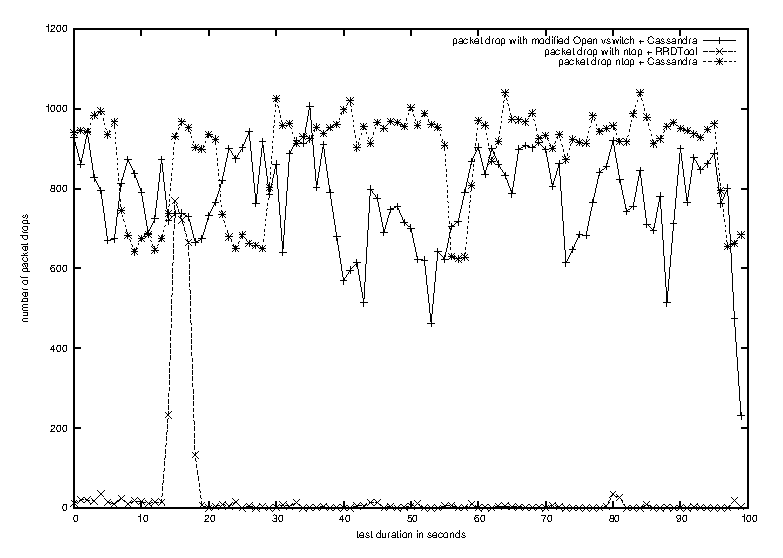
\includegraphics[scale=1]{data/out32}
	    \caption{Packet Drops with 32 KB Socket and IPC buffer size} 
	    \label{graph32}
	  \end{figure}
	
	  \begin{figure}[!htb]
	    \centering
	    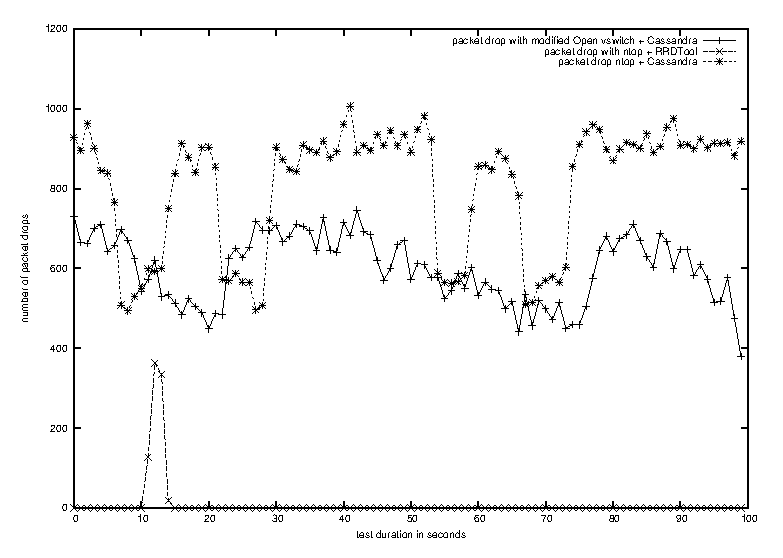
\includegraphics[scale=1]{data/out64}
	    \caption{Packet Drops with 64 KB Socket and IPC buffer size } 
	  \label{graph64}
	  \end{figure}
	  
	  \begin{figure}[!htb]
	    \centering
	    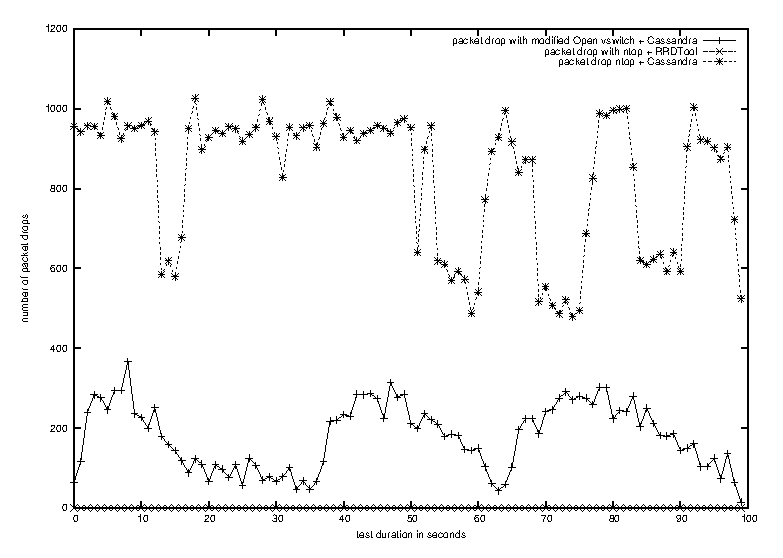
\includegraphics[scale=1]{data/out128}
	    \caption{Packet Drops with 128 KB Socket and IPC buffer size} 
	    \label{graph128}
	  \end{figure}
	  If we look at the detail operations that take place during our three tests, we may get more insights to analyze the results.
	  Operations done by \emph{ntop} with RRDTool:
	  \begin{enumerate}
	   \item Read NetFlow Packets from socket.
	   \item Analysis NetFlow packets 
	   \item Store NetFlow statistics into RRD with disk write.
	  \end{enumerate}
	  \emph{ntop} with Cassandra does similar operations except it stores NetFlow records into Cassandra using our Cassandra C client.
	  On the other hand Open vSwitch use \emph{Pycassa} to store NetFlow records into Cassandra. In both case, \emph{ntop} with RRDTool and Open vSwitch with Cassandra, a NetFlow packet pass thorugh network once and then stored into disk. In \emph{ntop} with Cassandra test, a Netflow packet has to pass through network twice, that explains why \emph{ntop} with Cassandra drops more packets than other two. \emph{ntop} with RRDTool is faster because RRDTool is written in c and dynamically linked with \emph{ntop}. Open vSwitch use Python, which is interpreted language and slower than
	  C.
	  \emph{ntop} with Cassandra does not improve its performance much with compare with Open vSwitch even we increase Socket buffer size.
	  \emph{ntop} uses our own Cassandra C client for storing data into Cassandra. Cassandra C client has pass through multiple layers of API calls (C-Python API, $Pycassa$ API, thrift API)	before reaching to Cassandra which is one reason for bad performance of \emph{ntop} with Cassandra. 
	  \paragraph\
	  
	  
	  

	  
\section{Conclusion} \label{Result_conclusion}
%\chapter{\label{chap:conclusion}Conclusions and Future Work}
%\input{conclusion.tex}
%\appendix
%\chapter{\label{chap:appendix} Design of the New Self-Organized Clustering Algorithm}
%\input{appendix.tex}
%\chapter{\label{chap:appendix} Modifications in \textit{ns-2} source code}
%\input{appendix_mod.tex}
\nocite{*}
\bibliographystyle{PhDbiblio-bold}
\newpage
\addcontentsline{toc}{chapter}{Bibliography}
\bibliography{ref.bib}
\newpage
\addcontentsline{toc}{chapter}{Index}
%\printindex
%\end{large}
\end{document}
